\documentclass[11pt, letterpaper]{article}

% --- Essential Packages ---
\usepackage[utf8]{inputenc}
\usepackage[T1]{fontenc}
\usepackage[margin=1in]{geometry} % Standard 1-inch margins
\usepackage{mathpazo} % Palatino font - looks more professional than default Computer Modern
\usepackage{microtype} % Improves text justification and spacing
\usepackage{setspace} % For line spacing
\usepackage{graphicx} % For images
\usepackage{amsmath, amssymb, amsfonts} % Standard math packages
\usepackage{booktabs} % For professional tables
\usepackage{hyperref} % Clickable links and refs
\usepackage[svgnames]{xcolor} % For colors
\usepackage{tikz}
\usetikzlibrary{shapes.geometric, arrows, positioning, fit, backgrounds}

% Define styles for the flow chart
\tikzset{
    sensor/.style={rectangle, draw=black!60, fill=blue!10, very thick, minimum size=1.5cm, align=center},
    process/.style={rectangle, draw=black!60, fill=orange!10, rounded corners, minimum height=1cm, align=center},
    model/.style={rectangle, draw=black!60, fill=green!10, very thick, minimum size=1.5cm, align=center},
    output/.style={rectangle, draw=black!60, fill=red!10, very thick, minimum size=1cm, align=center},
    arrow/.style={->, >=stealth, very thick}
}

% --- Bibliography Setup (using Natbib for Author-Year) ---
\usepackage[round, sort&compress]{natbib}
\bibliographystyle{plainnat}
% need to add \cite in all text then rm this
\nocite{*}
% --- Custom Header/Footer ---
\usepackage{fancyhdr}
\pagestyle{fancy}
\fancyhf{}
\lhead{\footnotesize \textbf{Research Proposal:} Physics-Informed GIC Prediction}
\rhead{\footnotesize [Your Name]}
\cfoot{\thepage}

% --- Section Formatting ---
\usepackage{titlesec}
\titleformat{\section}{\Large\bfseries\color{DarkBlue}}{\thesection}{1em}{}
\titleformat{\subsection}{\large\bfseries\color{DarkSlateGray}}{\thesubsection}{1em}{}

% --- Metadata ---
\title{\textbf{Physics-Informed Forecasting of Regional Geomagnetic Perturbations}\\
\large Integrating Solar Wind Coupling Functions across a Multi-Point Data Fusion Dataset}

\author{
    \textbf{Your Name} \\
    Master of Data Science Program \\
    University of California, San Diego \\
    \textit{Advisor/Mentor: [Advisor Name]}
}
\date{\today}

% --- Document Start ---
\begin{document}

\maketitle

% --- Abstract ---
\begin{abstract}
    \noindent Geomagnetically Induced Currents (GICs), driven by rapid fluctuations in the Earth's magnetic field ($dB/dt$), pose a significant risk to critical power infrastructure. While recent deep learning approaches have demonstrated predictive capability, they often function as "black boxes," lacking physical interpretability, or rely on curated datasets of isolated geomagnetic storms, introducing selection bias. This study proposes a novel "Gray Box" framework that fuses the architectural strengths of physics-informed neural networks with robust solar wind coupling physics. Unlike prior studies (e.g., Abduallah et al., 2024) that limit analysis to selected high-intensity events, this research utilizes a continuous, high-fidelity multi-point data fusion strategy. We integrate L1 solar wind measurements (ACE/DSCOVR), magnetospheric state data from GEO/LEO satellites, and ground magnetometer arrays (SuperMAG) from 2010 to 2025. This temporal range covers the entirety of Solar Cycle 24 and the rising phase of Cycle 25, mitigating quiet-time bias. By embedding physics-derived features; specifically Newell Coupling (representing magnetic reconnection efficiency and related state variables into the learning process, we aim to enhance model generalizability and quantify uncertainty. This approach directly addresses the lack of domain interpretability identified in recent literature and aligns with priority goals outlined in the 2024 SWAG Report and the 2024-2033 Heliophysics Decadal Survey.
\end{abstract}

% --- 1. Introduction ---
\section{Introduction}

\subsection{The Operational Imperative}
Space weather events, particularly those manifesting as Geomagnetically Induced Currents (GICs), represent a tier-1 threat to modern electrical grid infrastructure. The 2024 Space Weather Advisory Group (SWAG) report explicitly identifies a "shared demand for space weather forecasts that are more geographically specific (regionalized) and detailed (granular)". Current operational forecasting often relies on broad global indices (like Kp) which fail to capture the localized $dB/dt$ spikes that drive GICs at specific latitude thresholds. Furthermore, the electric power sector has identified that the current magnetometer network in North America is too geographically limited, forcing planners to rely on estimated field data that may not reflect reality.

\subsection{The Scientific Gap: From "Black Box" to "Gray Box"}
While deep learning (DL) has demonstrated superior predictive capabilities over traditional empirical models, the heliophysics community remains skeptical of pure "Black Box" approaches. As noted by Camporeale (2019), the clearest opportunity lies in creating forecasting models that are "built on both physics predictions and observed data". \newline \newline
A critical limitation in current literature (e.g., Abduallah et al.) is the reliance on curated datasets of isolated storms. This "event-based" training introduces a severe selection bias, effectively ignoring the "quiet time" dynamics that characterize the majority of the solar cycle. To achieve the "Systems-Based Research Approach" advocated by the 2025 Heliophysics Decadal Survey, models must move beyond isolated events and capture the continuous, self-consistent interactions between the solar driver and the Earth’s magnetosphere.

% --- 2. Background and Theory ---
\section{Background: A Multi-Point System Approach}

To address the "Mesoscale Challenge" and the lack of system-wide understanding, this study employs a multi-point data fusion strategy that treats the Sun-Earth connection as a coupled system rather than a simple input-output mapping.

\subsection{L1 Solar Wind: Upstream Driver}
Measurements from the Lagrange Point 1 (L1), provided by ACE and DSCOVR satellites, serve as the primary driver of the system. However, reliance solely on L1 data is insufficient due to propagation delays and the fact that OMNI data quality significantly declines when satellites drift outside $\sim60$ Earth radii ($R_E$). This necessitates rigorous cleaning and fusion with downstream sensors.

\subsection{Geosynchronous Orbit (GEO): Magnetospheric State}
A key innovation in this study is the inclusion of GOES magnetometer data (e.g., GOES-13/15). Sitting at $6.6 R_E$, these satellites act as an intermediate measure of the magnetospheric state. Physically, they measure magnetospheric compression ($B_z$) directly; when the solar wind strikes the magnetopause, GOES detects the compression before the ground stations register the spike[cite: 3]. This connects the L1 driver to the ground impact, turning the "Black Box" into an interpretable causal chain[cite: 4].

\subsection{Low Earth Orbit (LEO): The In-Situ Bridge}
To fully capture the system dynamics, we incorporate data from Low Earth Orbit (LEO), specifically the ESA Swarm constellation. While GEO monitors the magnetospheric boundaries, LEO satellites orbit directly within the ionosphere-thermosphere system—the "transition zone" where plasma physics shifts from collisionless to collisional regimes. The 2025 Decadal Survey identifies in-situ LEO data as a critical "untapped resource" for improving model accuracy. By measuring magnetic field perturbations and field-aligned currents (FACs) at this altitude, Swarm provides the missing link that maps the high-altitude magnetospheric compression (observed by GOES) to the specific regional perturbations detected on the ground.

\subsection{Ground-Based Impact: SuperMAG}
The final component of the system is the ground-based magnetometer array, accessed via SuperMAG. This aligns with the SWAG report's finding that "effective GIC mitigation... requires increased collaboration" and better utilization of ground-level measurements to validate vulnerability assessments.

\subsection{The Physics-Informed "Gray Box" Strategy}
Rather than forcing a neural network to learn Maxwell's equations from scratch, we inject domain knowledge directly into the model. We utilize the Newell Coupling function, which acts as a proxy for the rate of magnetic reconnection at the dayside magnetopause[cite: 6]. By explicitly providing the model with this "reconnection efficiency," we bridge the gap between pure physics models and data-driven inference, directly addressing the interpretability issues raised by the physics community.

% --- 3. Problem Statement ---
\section{Problem Statement}
Operational space weather forecasting currently faces a "Trilemma" of limitations that hinders reliable grid protection:

\begin{itemize}
    \item \textbf{The Distance Problem:} Reliance on single-point L1 monitors (ACE/DSCOVR) becomes unreliable when satellites drift significantly from the Sun-Earth line ($>60 R_E$), leading to unacceptably high false-alarm rates.
    \item \textbf{The "Black Box" Barrier:} While pure Deep Learning models have shown promise, they lack the physical interpretability required by operational centers. Conversely, empirical physics models often fail to capture the non-linear "memory" of magnetospheric energy accumulation.
    \item \textbf{Data Selection Bias:} Recent ML studies (e.g., Abduallah et al., 2024) frequently employ "event-based" training sets (e.g., $\approx 42$ isolated storms). This introduces severe "quiet-time bias," preventing models from learning the crucial transition dynamics between quiet and active states.
\end{itemize}

\begin{flushleft}
    Furthermore, current outputs are often global indices (Kp), which fail to meet the electrical power sector's specific need for \textit{regional} and \textit{localized} $dB/dt$ predictions.
\end{flushleft}

% --- 4. Research Questions ---
\section{Research Questions and Aims}
The primary aim of this research is to develop a \textbf{Physics-Informed "Gray Box" System} that bridges the gap between solar wind drivers and regional ground impacts. We formulate three specific questions to validate this approach:

\begin{enumerate}
    \item \textbf{The Physics Question:} Does the explicit injection of the \textbf{Newell Coupling function} into the model's latent space significantly reduce RMSE compared to purely data-driven "Black Box" baselines?
    \item \textbf{The "Sentinel" Question:} Does the fusion of intermediate \textbf{GEO (GOES)} and \textbf{LEO (Swarm)} data provide a statistically significant reduction in false positives compared to L1-only models, effectively acting as a "verification layer"?
    \item \textbf{The Bias Question:} Does training on a continuous, multi-cycle dataset (2010--2025) improve the model's ability to predict storm \textit{onset} compared to models trained solely on curated high-activity events?
\end{enumerate}

% --- 4. Methodology ---
\section{Methodology}

\subsection{Data Acquisition: A Multi-Point Constellation}
To overcome the "Distance Problem" of relying solely on L1 monitors, we construct a multi-point dataset spanning Solar Cycles 24 and 25 (2010--2025). This fusion integrates three distinct spatial layers:

\begin{enumerate}
    \item \textbf{Upstream Driver (L1):} Solar wind plasma and magnetic field data from ACE and DSCOVR. These monitors provide the upstream boundary conditions ($\sim1.5 \times 10^6$ km) with an approximate 30--60 minute propagation delay.
    \item \textbf{Magnetospheric State (GEO):} Magnetometer data from GOES-13/15 ($6.6 R_E$). As established in our preliminary study, these sensors capture magnetospheric compression on the dayside before the signal reaches the ground, serving as a critical verification layer for the L1 driver.
    \item \textbf{Ionospheric Interface (LEO):} High-resolution magnetic measurements from the Swarm constellation. Orbiting within the ionosphere, Swarm provides in-situ validation of field-aligned currents (FACs).
    \item \textbf{System Response (Ground):} Ground truth is derived from the SuperMAG array, specifically high-latitude stations (e.g., Abisko, Tromsø) most susceptible to auroral electrojet fluctuations.
\end{enumerate}

\subsection{Data Fusion and Preprocessing}
\label{sec:fusion}
Data from heterogeneous sources (different cadences and coordinate systems) will be unified into a single Master Dataset.

\subsubsection{Temporal Alignment and Imputation}
L1 and Ground data are typically 1-minute cadence, while Swarm operates at 1--50Hz. All high-frequency data will be downsampled to a 1-minute resolution using mean aggregation. To handle sensor dropouts without introducing artificial physics, we employ a "Safe Zone" imputation strategy validated in our feasibility phase:
\begin{itemize}
    \item \textbf{Gaps $< 5$ min:} Filled via linear interpolation, as solar wind density rarely changes discontinuously on this scale.
    \item \textbf{Gaps $> 30$ min:} Labeled as invalid. The time series is segmented into valid continuous "chunks" to prevent the LSTM from training on synthetic straight lines.
\end{itemize}

\subsubsection{Feature Engineering (The "Gray Box")}
To inject physical constraints into the model, we calculate the Newell Coupling Function ($\frac{d\Phi}{dt}$), which represents the rate of magnetic reconnection at the magnetopause:
\begin{equation}
    \frac{d\Phi}{dt} = v^{4/3}B_T^{2/3}\sin^{8/3}(\theta_c/2)
\end{equation}
Additionally, we compute the Magnetic Local Time (MLT) for GOES satellites. This allows the model to distinguish between "Daytime Compression" (a storm signal) and "Nighttime Stretching" (tail loading), resolving the geometric ambiguity inherent in raw magnetometer data.

\subsection{Model Architecture}
\label{sec:architecture}
Our feasibility analysis of the 2015 St. Patrick's Day storm demonstrated that "Snapshot" models (e.g., XGBoost) fail to capture the energy accumulation of the magnetosphere (Correlation $r=0.33$). Conversely, sequence-based models significantly improved performance ($r=0.55$). A Long Short-Term Memory (LSTM) network processes a historical window ($t_{-60} \to t_0$) of the fused state vector to predict the ground perturbation at $t_{+60}$. This architecture explicitly models the non-linear "memory" of the magnetosphere-ionosphere system.

% --- Insert TikZ Diagram ---
\begin{figure}[ht]
    \centering
    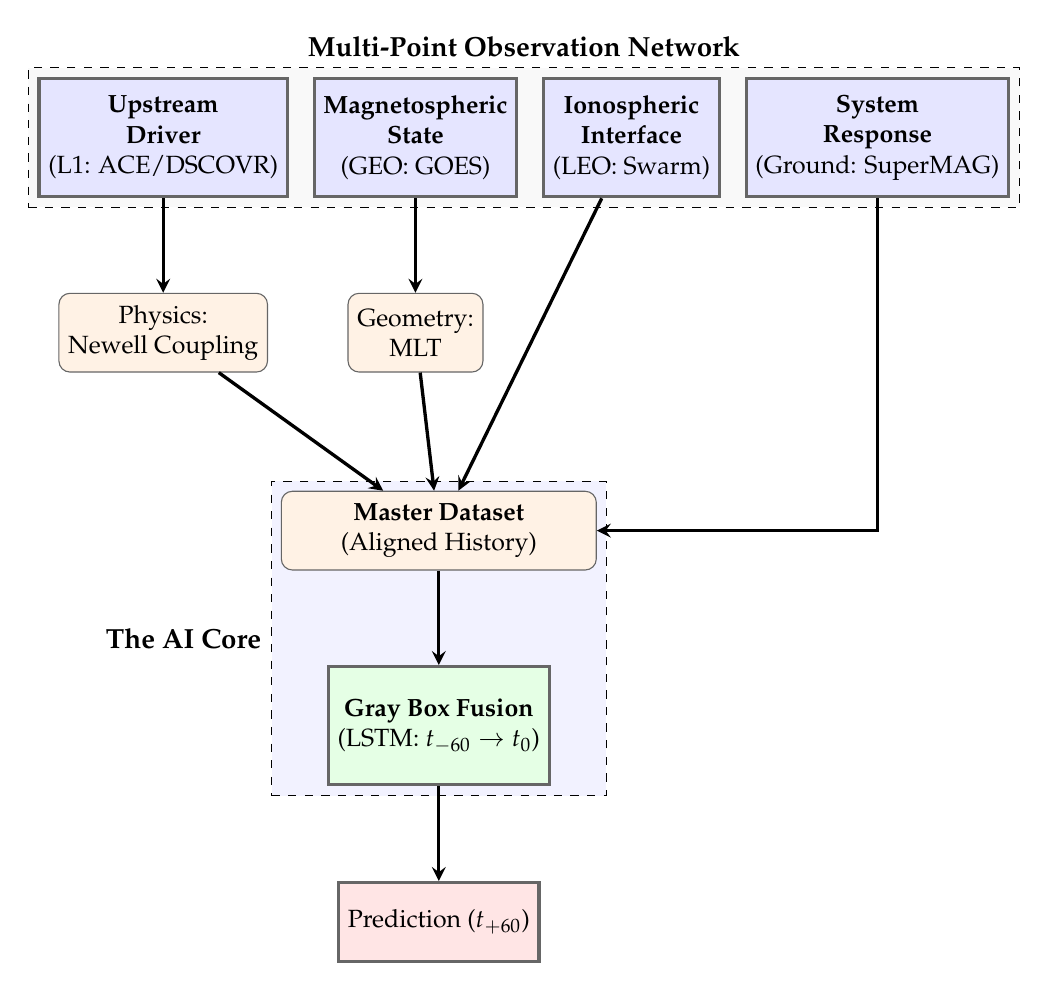
\begin{tikzpicture}[node distance=1.5cm]
        % --- Define Styles Locally (or keep in preamble) ---
        \tikzset{
            sensor/.style={rectangle, draw=black!60, fill=blue!10, very thick, minimum size=1.5cm, align=center, font=\small},
            process/.style={rectangle, draw=black!60, fill=orange!10, rounded corners, minimum height=1cm, align=center, font=\small},
            model/.style={rectangle, draw=black!60, fill=green!10, very thick, minimum size=1.5cm, align=center, font=\small},
            output/.style={rectangle, draw=black!60, fill=red!10, very thick, minimum size=1cm, align=center, font=\small},
            arrow/.style={->, >=stealth, very thick}
        }

        % --- Phase 1: Inputs with NEW NAMES ---
        % Note: I used double backslashes (\\) to stack the text so boxes don't get too wide.
        
        \node (L1) [sensor] {\textbf{Upstream} \\ \textbf{Driver} \\ (L1: ACE/DSCOVR)};
        
        \node (GOES) [sensor, right=0.3cm of L1] {\textbf{Magnetospheric} \\ \textbf{State} \\ (GEO: GOES)};
        
        \node (Swarm) [sensor, right=0.3cm of GOES] {\textbf{Ionospheric} \\ \textbf{Interface} \\ (LEO: Swarm)};
        
        \node (Ground) [sensor, right=0.3cm of Swarm] {\textbf{System} \\ \textbf{Response} \\ (Ground: SuperMAG)};
        
        % --- Phase 2: Processing ---
        \node (Physics) [process, below=1.2cm of L1] {Physics: \\ Newell Coupling};
        \node (Geom) [process, below=1.2cm of GOES] {Geometry: \\ MLT};
        
        % --- Phase 3: Fusion ---
        % Increased width to catch both inputs nicely
        \node (Master) [process, below=1.5cm of Physics, xshift=3.5cm, minimum width=4cm] {\textbf{Master Dataset} \\ (Aligned History)};
        
        % --- Phase 4: Model ---
        \node (LSTM) [model, below=1.2cm of Master] {\textbf{Gray Box Fusion} \\ (LSTM: $t_{-60} \to t_0$)};
        
        % --- Phase 5: Output ---
        \node (Prediction) [output, below=1.2cm of LSTM] {Prediction ($t_{+60}$)};
        
        % --- Arrows ---
        \draw [arrow] (L1) -- (Physics);
        \draw [arrow] (GOES) -- (Geom);
        
        % Direct connection into the Master box
        \draw [arrow] (Physics) -- (Master);
        \draw [arrow] (Geom) -- (Master);
        
        % Side connections for LEO and Ground
        \draw [arrow] (Swarm) -- (Master);
        \draw [arrow] (Ground) |- (Master);
        
        \draw [arrow] (Master) -- (LSTM);
        \draw [arrow] (LSTM) -- (Prediction);
        
        % --- Background Boxes ---
        \begin{pgfonlayer}{background}
            \node [fit=(L1) (Ground), fill=gray!5, draw, dashed, label=above:\textbf{Multi-Point Observation Network}] {};
            \node [fit=(Master) (LSTM), fill=blue!5, draw, dashed, label=left:\textbf{The AI Core}] {};
        \end{pgfonlayer}
    \end{tikzpicture}
    \caption{Proposed System Architecture using a Multi-Point Observation Network. The pipeline fuses the Upstream Driver (L1), Magnetospheric State (GEO), and Ionospheric Interface (LEO) to predict the System Response (Ground).}
    \label{fig:architecture}
\end{figure}

\subsection{Evaluation Strategy}
To address the "Conservative Bias" identified in preliminary testing (where models under-predict extreme spikes), we will implement a Weighted Mean Squared Error (WMSE) loss function. This function applies higher penalties to errors occurring during active storm times ($dB/dt > \text{threshold}$), forcing the model to prioritize storm onset detection over quiet-time accuracy.

% --- 5. Literature Review ---
\section{Literature Review}

\subsection{Deep Learning in Heliophysics: The "Black Box" Era}
The shift from empirical physics models to data-driven approaches has accelerated significantly in the last five years. Chen et al. (2019) demonstrated the efficacy of Convolutional Neural Networks (CNNs) for predicting geomagnetic storms, outperforming traditional linear regression models. More recently, Thaker et al. (2025) illustrated that deep learning architectures can effectively map solar wind parameters to ground perturbations. However, these models often suffer from a lack of interpretability. As noted by Camporeale (2019), the physics community remains skeptical of "Black Box" operational tools. Camporeale argues that the clearest path forward is the "Gray Box" approach: architectures that explicitly embed physical laws (e.g., Maxwell's equations or coupling functions) into the learning process to ensure physical consistency.

\subsection{The Bias and Reliability Challenge}
A critical flaw in current ML literature is the reliance on curated "event-based" datasets. For example, Abduallah et al. (2024) trained models on a subset of approx. 42 high-intensity storms. While this yields high accuracy metrics during peak activity, it introduces severe "quiet-time bias," causing the model to generate excessive false positives during nominal conditions. The reliability of the input driver itself is often overlooked. Vokhmyanin et al. (2019) established that L1 monitors (ACE/DSCOVR) lose significant predictive power when their orbital position drifts $>60 R_E$ from the Sun-Earth line. Standard "Black Box" models blindly accept this degraded data, whereas a physics-aware system must account for these geometric reliability gates.

% --- 6. Significance ---
\section{Significance and Impact}

\subsection{Alignment with National Priorities}
This research directly addresses the "Overarching Theme 1" of the 2024 Space Weather Advisory Group (SWAG) Report, which identifies a critical user need for "regionalized and granular" forecasts rather than global averages. By utilizing the high-latitude SuperMAG stations as explicit targets, this project moves away from global indices (Kp) to actionable, local $dB/dt$ predictions required by the electric power sector.

\subsection{Scientific Contribution: The Systems Approach}
The 2025 Heliophysics Decadal Survey calls for a "Systems-Based Research Approach" that treats the Sun-Earth environment as a coupled system rather than isolated data points. This work answers that call by:
\begin{itemize}
    \item \textbf{Bridging the Gap:} Fusing LEO (Ionospheric Interface) and GEO (Magnetospheric State) data to solve the "Mesoscale Challenge" of understanding intermediate structures.
    \item \textbf{Operationalizing Physics:} Proving that "Gray Box" methods can satisfy both the accuracy requirements of data scientists and the interpretability requirements of space physicists.
\end{itemize}

% --- 7. Timeline ---
\section{Project Timeline}
The proposed research is structured as a 16-week sprint, leveraging the preliminary feasibility analysis already conducted.

\begin{itemize}
    \item \textbf{Phase 1: Data Infrastructure (Weeks 1--4)}
    \begin{itemize}
        \item Acquire full continuous datasets (2010--2025) for ACE, DSCOVR, GOES, Swarm, and SuperMAG.
        \item Implement the "Safe Zone" imputation strategy (linear interpolation for gaps $<5$ min; segmentation for gaps $>30$ min).
        \item \textit{Milestone:} Delivery of the "Master HDF5 Dataset" (approx. 50GB).
    \end{itemize}
    
    \item \textbf{Phase 2: Physics Injection \& Architecture (Weeks 5--8)}
    \begin{itemize}
        \item Engineer physics features: Newell Coupling, Borovsky Coupling, and Clock Angles.
        \item Construct the "Gray Box" LSTM architecture with separate input heads for L1 (Driver) and GEO/LEO (State).
        \item \textit{Milestone:} Baseline XGBoost vs. LSTM comparison complete.
    \end{itemize}
    
    \item \textbf{Phase 3: Training \& Validation (Weeks 9--12)}
    \begin{itemize}
        \item Train on Solar Cycle 24 (2010--2019); Test on Cycle 25 (2020--2025).
        \item Implement Weighted MSE loss to penalize "missed storms."
        \item Conduct "Quiet Time" analysis to verify false positive reduction (The Vokhmyanin Check).
    \end{itemize}
    
    \item \textbf{Phase 4: Analysis \& Writing (Weeks 13--16)}
    \begin{itemize}
        \item Generate "GIC Risk Maps" for the St. Patrick's Day storm (Case Study).
        \item Finalize paper.
    \end{itemize}
\end{itemize}

\section{To do}
\begin{itemize}
    \item gather all sources and add to \texttt{references.bib}
    \begin{itemize}
        \item fill out many more literature review TLDR points
        \item adjust \textit{5.4 Evaluation Strategy} based on previous work
        \item refine significance and impact
        \item mo' sources mo' problems: add/refine to \textit{3 Problem Statement}
    \end{itemize}
    \item buff and polish.. get the horse hairs out
    \item add data descriptions from the cdwa website??
    \item blue box, green box, gray box: iron this out since i think gray box is standard practice (IMPORTANT)
\end{itemize}

% --- References ---
\nocite{*}
\bibliography{references} % Points to references.bib

\end{document}
